% !Mode:: "TeX:UTF-8"
\chapter{Introduction}

Nowadays there are many existing image compression approaches. We can divide such algorithms in two groups: lossy (such as JPEG. Mainly such algorithms use Discrete Cosine Transform) and lossless (such as DEFLATE. Mainly such algorithms use similar to Huffman Encoding methods). Both have been developed for decades already. It is important to mention that image containers (such as JPEG, PNG, GIF etc.) are using information compression algorithms \textit{only as a part} of their architecture. Usually lossy and lossless compression methods are combined to achieve higher performance.

\section{Traditional image compression pipeline and JPEG as an example}

JPEG is widely used in image compression applications. It was introduced in 1992 \cite{wallace_jpeg_1992}. Algorithm consists of several steps.

\begin{enumerate}
    \item Transformation from RGB to YCbCr (Chroma subsampling).
    \item Discrete Cosine Transform. Lossless.
    \item Quantization. Lossy.
    \item Coding. Lossless.
\end{enumerate}

\subsection{Compression algorithm}

Chroma subsampling is a process of transformations from RGB format to YCbCr. YCbCr is a special format of storing image data not in Red, Green and Blue channels, but in Y, Cb and Cr channels. Y is the brightness channel of an image, Cb is the blue difference relative to the green color, Cr is the red difference relative to the green channel. After that it is already possible to reduce size by rescaling Cb and Cr channels by four. By doing so, the space is reduced by 1.5.

Compression of each channel is an performed in parallel. Image is partitioned into blocks 8x8 pixels. Each block is processed independently. Block values are centered at 0, so the values are in range (-127, 127). Then Discrete Cosine Transform (DCT) is being applied.

We can view an image as a combination of different frequencies. Pixel values can vary over given image, and we view this variation as a periodic function $f(x, y)$ where $x$ is horizontal coordinate and $y$ is a vertical one. There is a matrix of DCT coefficients, which consists of elements of different frequencies from low frequencies to high. High frequencies can be omitted to achieve better compression performance.

Mathematically, the DCT is one-to-one mapping for 64-point vectors between the image and the frequency domains. If the FDCT (Fast Discrete Cosine Transform) and IDCT could be computed with perfect accuracy and if the DCT coefficients were not quantized as in the following description, the original 64-point signal could be exactly recovered. In principle, the DCT introduces no loss to the source image samples; it merely transforms them to a domain in which they can be more efficiently encoded.

Each element of obtained matrix is a coefficient of corresponding frequency. Basically, the meaning of an element of this matrix is how much of this frequency is in given image. Then goes quantization, this step is lossy, and on this step elements of coefficients matrix are divided by so called standard JPEG quantization table. By the end of this procedure we have a matrix with coefficients. Relatively small coefficients can be omitted to react higher compression performance, since their frequencies contribution to image are tiny. Quantization table is specified as an input by application or user. Each element of quantization table is a number in range $(0; 255)$ which specifies the step size of the quantizer for its' corresponding DCT coefficient.

\begin{equation}
    \label{eq:00}
    F(u,v)=\dfrac{1}{4}C(u)C(v)[\sum_{x=0}^{7}\sum_{y=0}^{7}{f(x,y)*cos(\dfrac{(2x+1)u\pi}{16})*cos(\dfrac{(2x+1)v\pi}{16})}]
\end{equation}

\begin{equation}
    \label{eq:01}
    f(x,y)=\dfrac{1}{4}[\sum_{x=0}^{7}\sum_{y=0}^{7}{C(u)C(v)F(u,v)*cos(\dfrac{(2x+1)u\pi}{16})*cos(\dfrac{(2x+1)v\pi}{16})}]
\end{equation}

where:

\begin{equation}
    \label{eq:02}
    \begin{split}
        C(u), C(v) = \dfrac{1}{\sqrt{2}} \text{for } u,v=0 \\
        C(u), C(v) = 1 \text{otherwise}
    \end{split}
\end{equation}

Huffman coding is a type of entropy coding algorithms. This algorithm performs coding based on frequencies of each symbol in sequence. The goal is to encode most frequent symbols using less bits of information, since they appear in sequence more. Less frequent symbols are encoded using more bits of information since they appear in sequence less.

The result of Huffman coding is a Huffman tree \ref{huffman-tree}. To build this tree we need to follow the steps:

\begin{enumerate}
    \item Calculate frequencies of each symbol in sequence.
    \item Sort symbols in increasing order of frequencies.
    \item Make each unique symbol a leaf node (in other words, independent tree).
    \item Create an empty node and attach two leafs with smallest frequencies to this node as a children.
    \item Set value of this new node as a sum of it's children frequencies.
    \item Repeat steps 4-5 until thee is built.
    \item Each left edge must be labeled as $0$, each right edge must be labeled as $1$.
    \item Each symbol can be encoded using a path from the root node of a tree to this symbol.
\end{enumerate}

\begin{figure}[!ht]
    \centering
    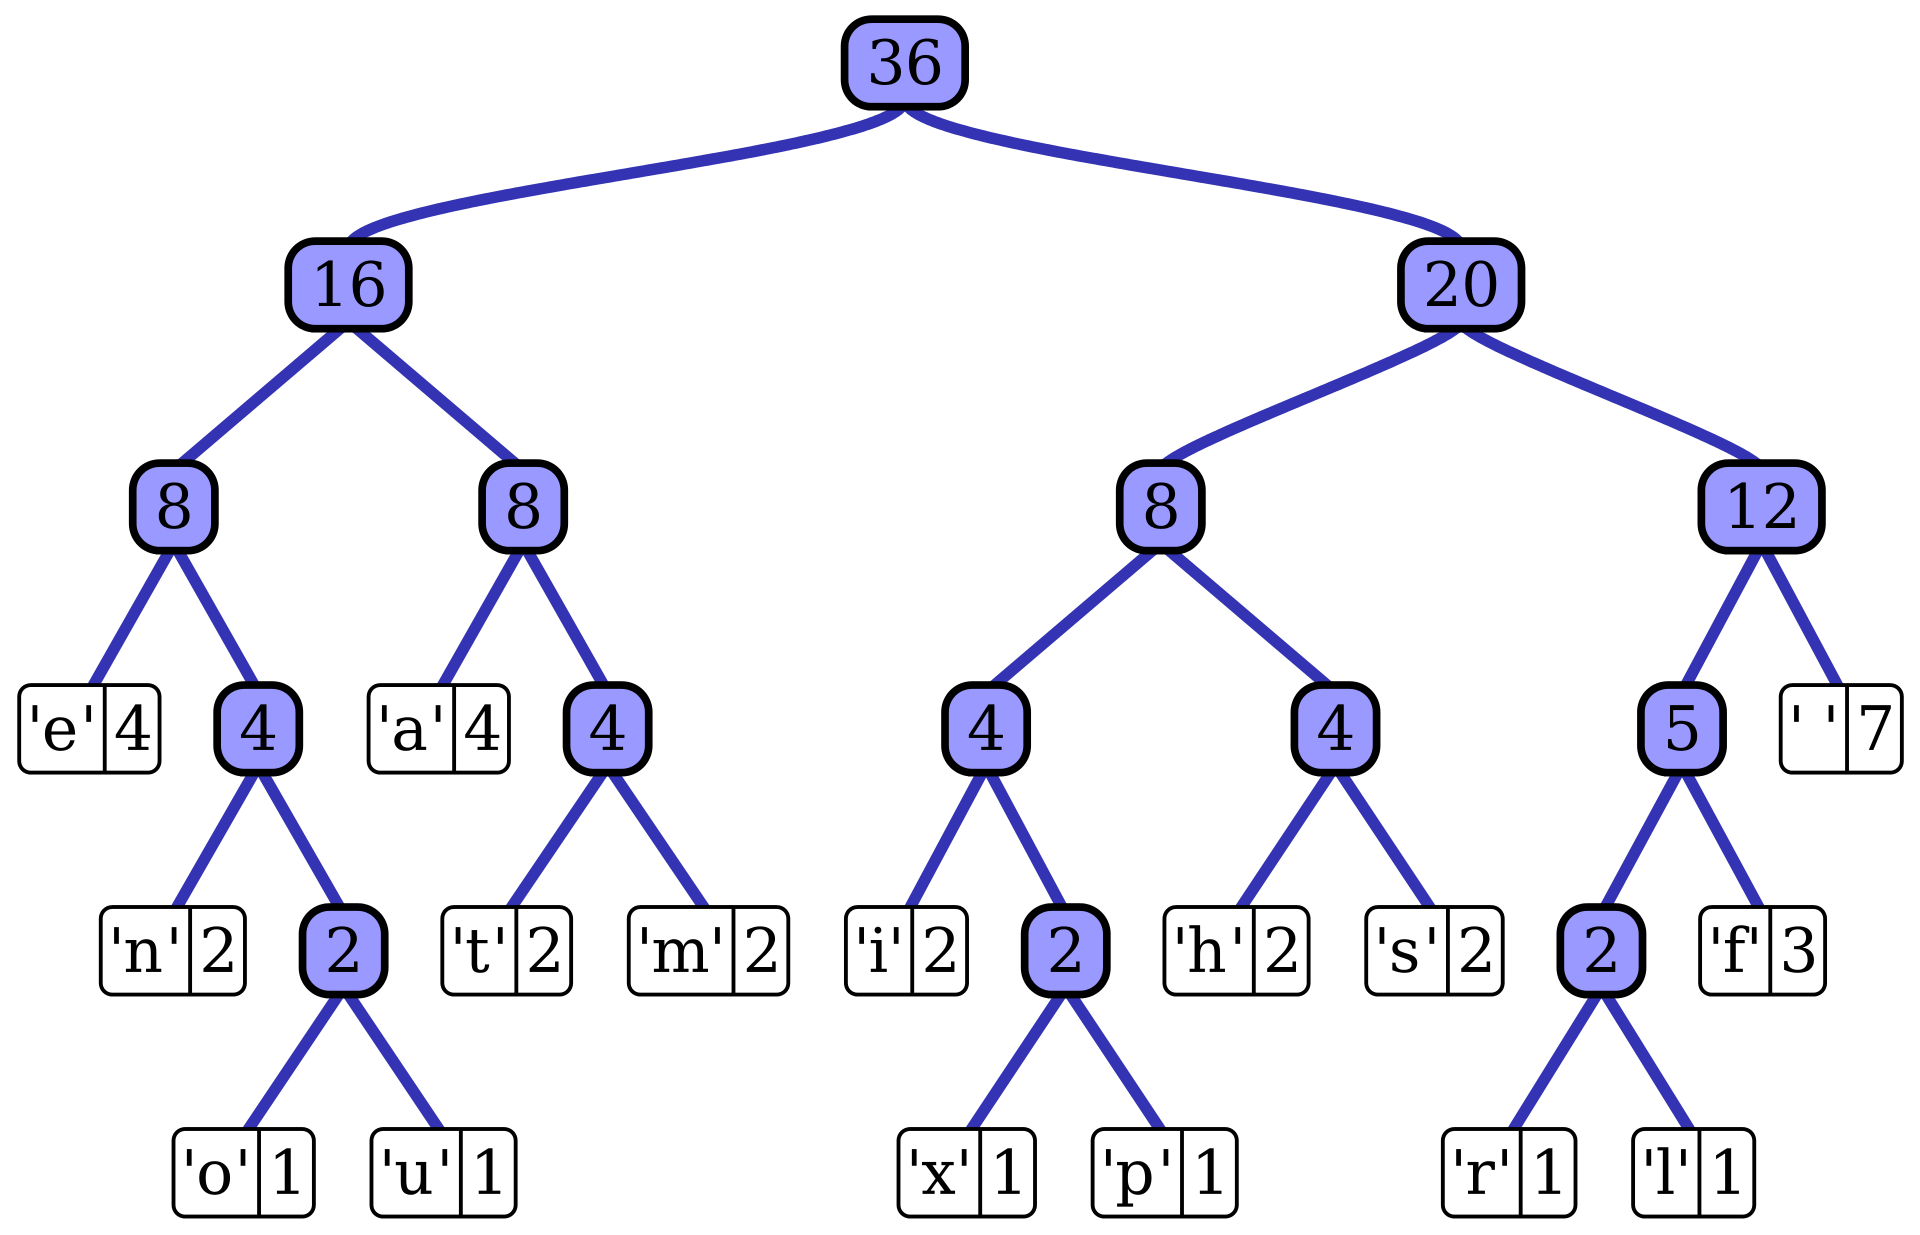
\includegraphics[width=\textwidth]{figure/Huffman_tree_2.svg.png}
    \caption{Huffman tree is a special type of binary tree. Each node of this tree can be described as a path from the root. This path consists of choices: left or right, which are encoded using ${0, 1}$}
    \label{huffman-tree}
\end{figure}

Huffman coding is performed on matrix obtained after DCT and quantization. this matrix is being reshaped to linear sequence (it is called Zig-Zag sequence, since the trajectory has a shape of zig-zag from top left corner up-down to the bottom-right corner).

\subsection{Decompression}

Decoding process consists of several steps, which are basically a reversed encoding steps.

\begin{enumerate}
    \item Decoding. Lossless.
    \item Dequantization. Lossy.
    \item Inverse Discrete Cosine Transform. Lossless.
    \item Transformation from YCbCr to RGB.
\end{enumerate}

To restore initial image first each block is passed through Huffman decoding algorithm. This step is lossless, so it just transforms a number with frequencies to a matrix obtained after DCT (during compression process).

For decoding Huffman codes it's required to take a code of the symbol and traverse through the Huffman tree. By the end of one traverse (in other words - reaching a leaf node), an original symbol is being obtained. So we can get a quantized coefficients matrix. To further continue decoding process dequantization is applied.

Dequantization is the inverse operation of quantization. Here it means that normalization is removed by multiplying by step size, which is specified in quantization table. To remind, this table is selected as an input information for the whole compression process before compression, and this is exactly same table as the one that was used during encoding process.

The next step is IDCT (Inverse Discrete Cosine Transform). IDCT takes the 64 DCT coefficients (which at that point have been quantized) and reconstructs a 64-point output image signal by summing the basis signals.

The last step of decompression is transformation from YCbCr representation to RGB. Ths transformation is a simple arithmetic which we omit here.

TODO: formulas here

All these steps are reversible, which makes this algorithm stable and convenient to use in image compression. However, it has a couple of problems. One of these problems is an effective size of compressed image, as well as quality and consistency of compressed image. JPEG compression was introduced long time ago when computational power was not enough to perform calculations with high computational costs. At that time lightweight and rapid algorithm was needed to satisfy industry need. Now it is not necessary true. Modern compression approaches of course include a computationally expensive compression algorithms, such as neural compression.

\section{Modern approaches}

There is a certain trend to apply a power of neural networks in compression domain, extending a group of lossy algorithms. First approaches were \cite{Balle_Laparra_Simoncelli_2017}, \cite{Theis_Shi_Cunningham_Huszar_2017}, \cite{Toderici_Vincent_Johnston_Hwang_Minnen_Shor_Covell_2017}, where authors proved that it is possible to use one neural network to generate a compressed representation of an image and another neural network to restore initial image from its representation generated by first network. Now such networks are also being used to solve an image and video upscale tasks.

Recent progress in neural image compression has shown a great progress:

\begin{enumerate}
    \item Now image neural image compression outperform traditional compression algorithms such as JPEG and JPEG2000.
    \item Autoencoder architecture can be extended with different compression modules in between.
    \item Development of convolutional layers architecture provides a more powerful tools to extract image features and reconstruct initial image.
\end{enumerate}

However, several issues are still remaining unsolved:

\begin{enumerate}
    \item False textures.
    \item Limited compression power.
    \item Fixed output size.
\end{enumerate}

We separate neural image compression to two main groups:

\begin{enumerate}
    \item Methods that follow traditional image compression pipeline, while changing some part of it.
    \item Methods that create a new pipeline, while using some parts from traditional pipeline.
\end{enumerate}

For now a general approach is to encode an image to compressed representation using convolutional neural network and take the convolutional features from one of the top layers of network. In this work we are going to use a slightly different architecture.

In this work we are going to apply fully convolutional neural network to extract features from given image, compress those features using another encoder and arithmetic coding algorithm. Then this compressed representation will be restored using decoder and upsample modules. It worth to mention that the algorithm we are working on is lossy. Our method will combine traditional image compression approaches and neural network image compression approach.

\chapter{Objective}

Our motivation is that traditional image compression methods are simple and computationally efficient. However, using more heavy neural models we can compress image much more efficient. By combining these two methods we can reach equilibrium.

Nowadays existing methods have a strong compression power. Existing models significantly overcome traditional methods by many metrics. The most impressive though is a PSNR metrics, which measures an effectiveness of compression. From the figure we can see a comparison of JPEG and famous HiFiC \cite{mentzer_high_fidelity_2020}

\begin{figure}[!ht]
    \centering
    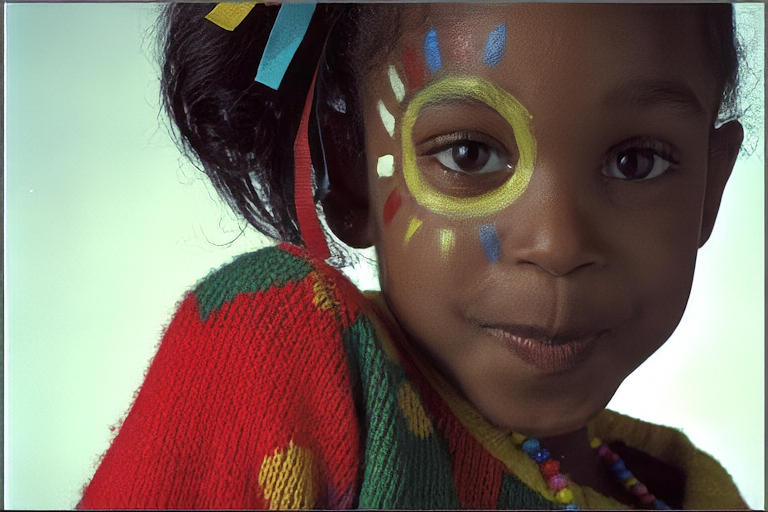
\includegraphics[width=.45\textwidth]{figure/kodim15_HiFiC_Lo.png}
    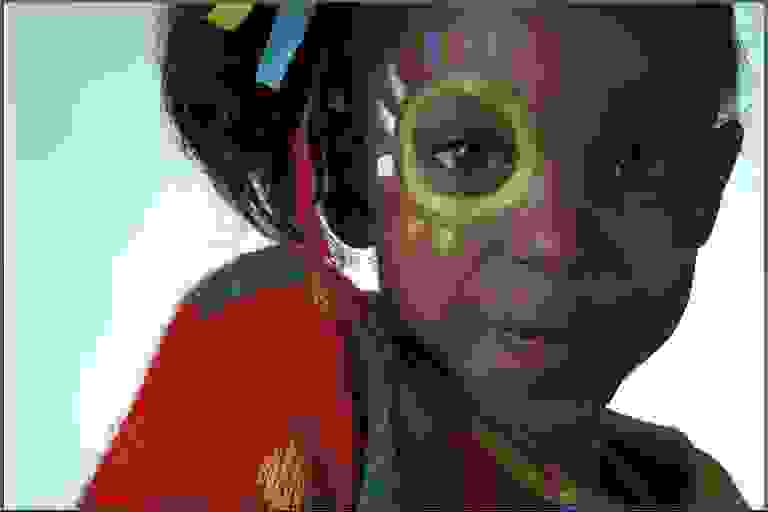
\includegraphics[width=.45\textwidth]{figure/kodim15_jpg_1x_0.166.jpg}
    \caption{}
    \label{jpeg-hific-comparision}
\end{figure}

Image can be represented using a convolutional features and we can train two neural networks to extract features from given image and reconstruct initial image from these features back. Such a network should have an encoder and a decoder. Encoder is trained to extract meaningful information form given image, which we call feature map or latents; Decoder is trained to reconstruct initial image given latents. We can train such system simply by penalizing L1 or L2 distance between given image and its reconstruction.

\begin{equation}
    \label{eq:1}
    L1=\sum \hat{I}-I
\end{equation}

These intermediate convolutional features already take less disk space than raw initial image. However, we can compress these features using lossless coding algorithm. We are using arithmetic coding because of its huge capacity to compress sequences of numerical values.

It is not difficult to train an autoencoder to compress some information and decompress it back. So, we are using the same design as \cite{Ballé_Minnen_Singh_Hwang_Johnston_2018} to compress hidden features and obtain hyperlatents. Then they can be encoded by lossless compression algorithm.

After compressing image we need to be able to decompress these hyperlatent features back. Say we used lossless coding algorithm to decode hyperlatents, passed them to Hyperprior decoder and get latents. Then we feed these latents to fully convolutional decoder and apply deconvolution operation several times together with upscaling layers to make resulting image bigger. Finally we pass it through several super resolution layers to obtain an image with reduced blur artifacts, more sharp structure and, if needed, higher spacial resolution.

Such a system is complicated and since we need to train it efficiently, we consider using generative adversarial training pipeline to fit the model to data. Discriminator will be trained to till real and generated images apart, which will stabilize training.

\chapter{Niches}

Potentially this work can improve existing image compression algorithms. The disk space required to store hyperlatents is less than disk space required to store raw images or even images encoded with JPEG or JPEG2000. Such an algorithm can be used in different scenarios. Mainly we can use it in traditional use cases for lossy compression such as using it in image format as it is or in more advance sense, to extend existing formats. For example we can extend existing DCT (Discrete Cosine Transform) or DWT (Discrete Wavelet Transform). We selected two possible use cases to apply the compression algorithm we are developing:

\begin{enumerate}
    \item Limited space on machine with high computational power. It can be a big server with powerful CPU. In recent days there are some movements in quantum computing sphere, so it can be a very powerful machine with quantum CPU etc.
    \item Huge images needed to be transmitted through a network with limited speed. In case of a limited performance of a network we can compress and restore images using application, we are working on.
\end{enumerate}

Few years ago already a reasonable performance has been achieved using an encoder-decoder architecture \cite{Theis_Shi_Cunningham_Huszar_2017}. We suppose, that our approach can boost performance both in sense of visual appearance and sense of compressed image size.

The contribution of this work can be considered from two major perspective. The first is that this work is the first approach to use super resolution methods in decoder architecture. From the second perspective we are going to use a general autoencoder architecture together with compression and coding algorithms. And finally our work proposes a new way of thinking of image compression: since we are using fully convolutional neural networks through the whole pipeline of our algorithm, and in decoder we are using upscale layers, user is able to select a size (or scaling factor) of produced images.

\chapter{Methodology}

In our work we compared several approaches to compress images. At first we tried to use a graph as a representation of an image. This approach is quite intuitive, since graph has a certain information about image structure. However, after series of experiments, we figure out that graph cannot represent image identity precisely. And most importantly, current state of the art methods are not capable of producing a good image from a scene graph, since scene graph to image architectures use scene graph to scene layout to image architecture, which makes scene graph a redundant information and only makes reconstructed images worse. We also found out that layout to image algorithms such as \cite{Zhao_Meng_Yin_Sigal_2019} use LSTM network architecture to fuse layout objects into singe representation, but LSTM is not designed to capture spatial relations and fuse objects into single one, since layout objects are unordered. In future this task can be potentially solved by using permutation invariant fusion module.

\section{Autoencoder}

Autoencoder is a popular architecture for neural networks. It has been first introduced in \cite{HinSal06} and proven to be a powerful tool in dimensionality reduction tasks. Basically, autoencoders were introduced to solve a particular problem of dimensionality reduction. The goal of an original autoencoder is to reduce dimensionality of input tensor. PCA (principal component analysis) is a widely used method to perform a dimensionality reduction. PCA finds the directions of greatest variance over a dataset, and then represents each point in a dataset by its coordinates along these directions. These directions are called principal components and the number of principal components is significantly less than number of components of original data point.

PCA uses a statistical approach to fit data. More precise, PCA is based on Eigen-decomposition, where we find a matrix of eigenvectors and eigenvalues of the covariance matrix and take $N$ biggest eigenvalues and $N$ corresponding eigenvectors. These are called principal components.

Similarly to PCA, autoencoder reduces dimensionality of an original data point, but the core principle of autoencoder is different from PCA. Instead of having a fixed algorithm to reduce dimensionality, autoencoders employs a power of neural networks. Autoencoder has two networks: encoder and decoder. Encoder is a network that embeds an original data into space with much smaller dimensions by sequentially passing original data through convolutional layers. These layers reduce dimensions of data, keeping however the most significant information. After the encoder, reduced features go through decoder, which increases dimensionality of data to its' original shape.

\begin{figure}[!ht]
    \centering
    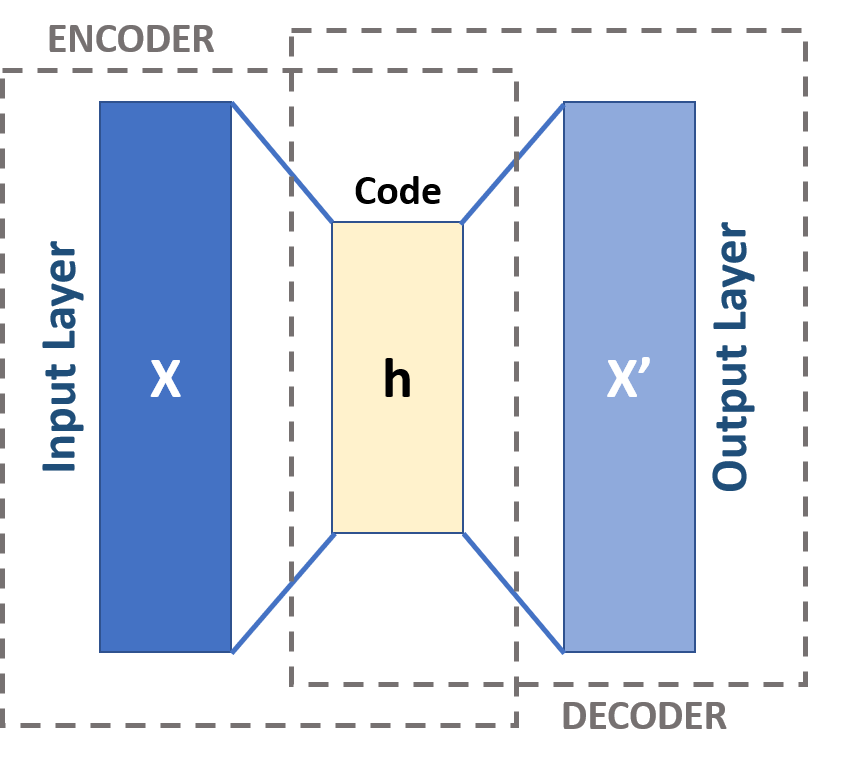
\includegraphics[width=\textwidth]{figure/Autoencoder_schema.png}
    \caption{Autoencoder schema.}
    \label{autoencoder-schema}
\end{figure}

Autoencoder is trained in supervised manner: feed data, pass it through encoder and decoder, calculate difference between original image in the output, then back propagate. After sufficient amount of iterations autoencoder finds its' local minimum. At this moment we need to stop training process, store weights and fix them.

Autoencoders have many applications \ref{autoencoder-popularity-stats} in compression, denoising, debluring, upscaling etc. The conceptual idea in all these applications is that hidden representation is a compressed version of input data, then original data is restored by generator. The loss here is significant since this is actually the criteria of autoencoder performance and for different tasks the criteria is formulated differently.


TODO: difference between these models

\begin{figure}[!ht]
    \centering
    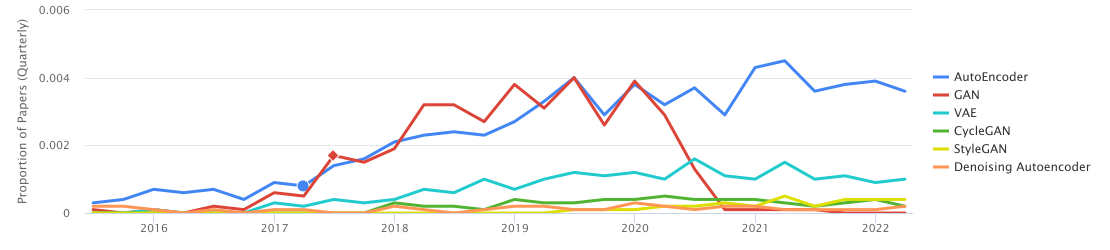
\includegraphics[width=\textwidth]{figure/autoencoder-popularity-over-time.png}
    \caption{Autoencoder architecture popularity over time compared to other popular neural network architectures (data from paperswithcode \cite{autoencoder_papers})}
    \label{autoencoder-popularity-dynamics}
\end{figure}

TODO: About autoencoder application and spheres of applications.

\begin{figure}[!ht]
    \centering
    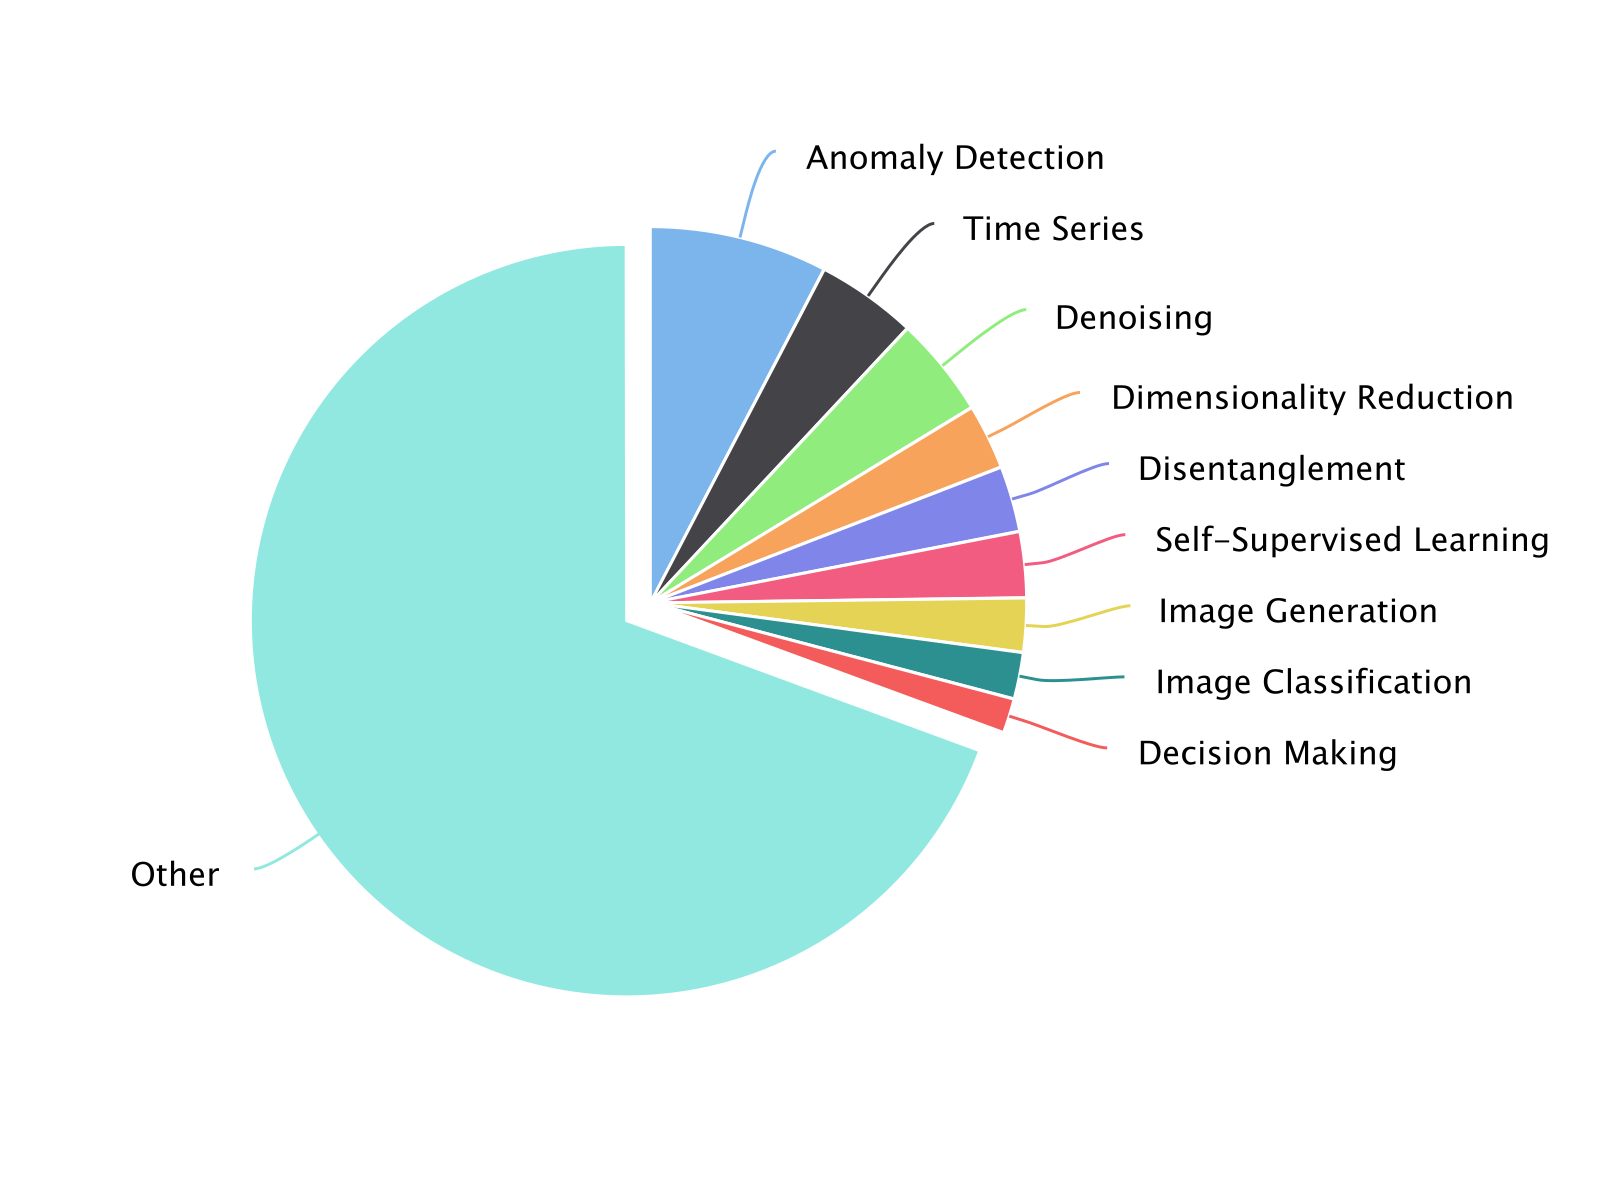
\includegraphics[width=\textwidth]{figure/autoencoder-popularity-stats.png}
    \caption{Autoencoder architecture usage statistics by paper' subject (data from paperwithcode website \cite{autoencoder_papers})}
    \label{autoencoder-popularity-stats}
\end{figure}

We use fully convolutional neural networks (FCN) in the encoder \ref{encoder}. FCNs are a family of convolutional neural networks which does not use pooling layers or bilinear interpolation or any other layer that can cause an information loss. Layers like pooling layer only propagate one value though itself. It causes a situation when we cannot determine or learn any information about input to this layer knowing it's output.

\subsection{Encoder}

Let us consider a pooling layer as an example to make our concern clear. Pooling layer takes a patch from an image (or from a feature map) and aggregates all those values into single output value. Pooling layers usually make use of aggregation functions such as \textit{max}, \textit{min}, \textit{avg} etc. Those functions are permutation invariant, which means we cannot reverse them. Even in theory it is impossible to get an inverse functions for pooling layers kernels, since pooling operation causes information loss.

\begin{figure}[!ht]
    \centering
    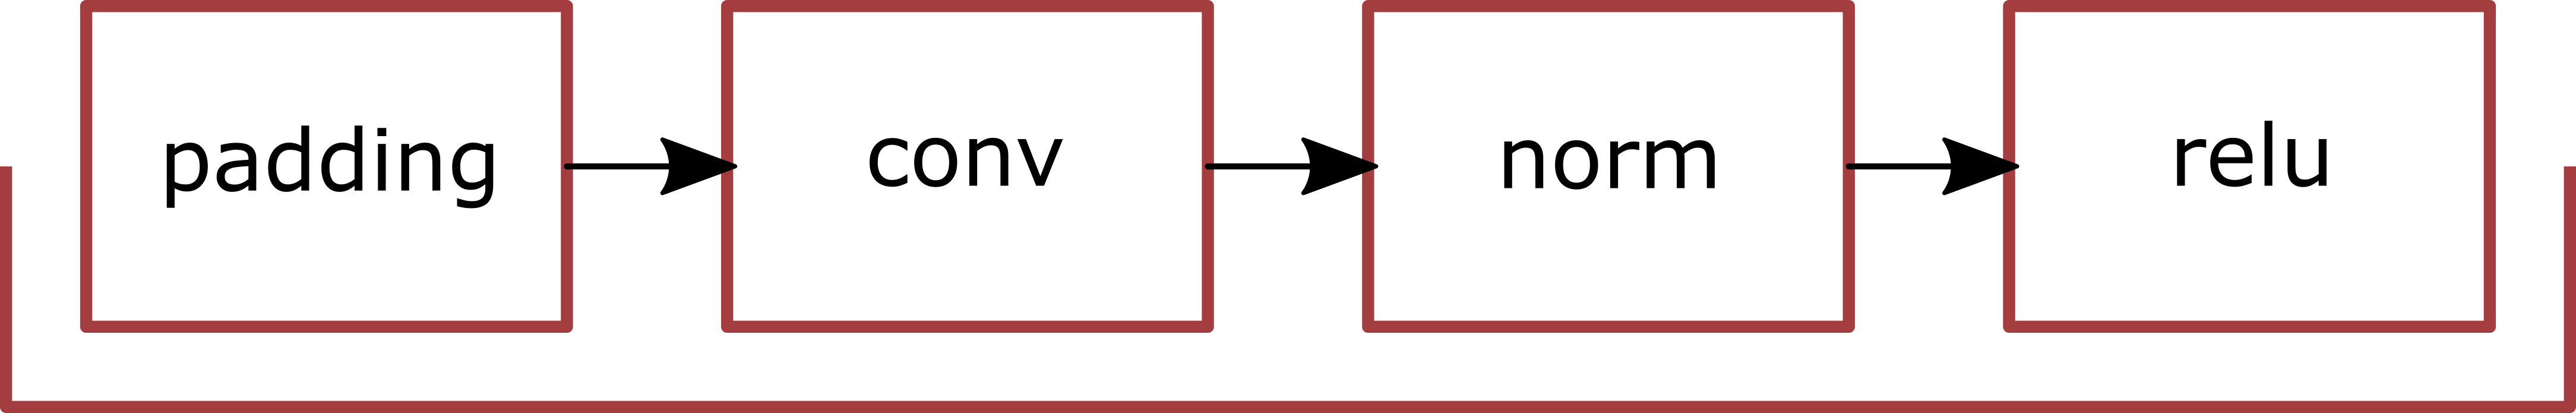
\includegraphics[width=\textwidth]{figure/encoder.png}
    \caption{Convolutional block of the encoder. We stack 6 such blocks to obtain encoder.}
    \label{encoder}
\end{figure}

\subsection{Decoder}

After a motivation for using FCNs in our encoder, let us take a look on the decoder \ref{decoder}. And the logic here is absolutely same: To restore an image given hidden feature map we need to learn an inverse function, which can be only obtained by reverse of encoder. In practice it means that we need both encoder and decoder to be FCNs \ref{autoencoder}. It will make the entire pipeline less lossy and make an intermediate features more interpretable, since using only convolutional layers helps to achieve a certain consistency in mapping features from input of one layer to its output.

\begin{figure}[!ht]
    \centering
    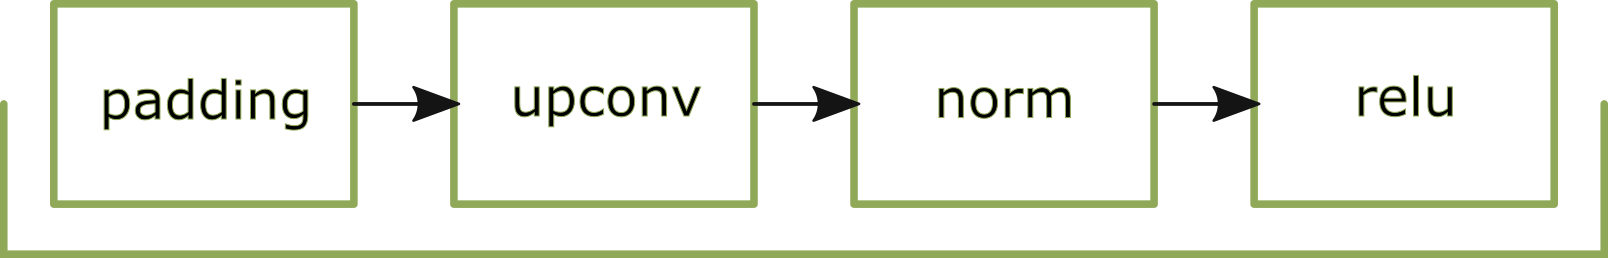
\includegraphics[width=\textwidth]{figure/generator.png}
    \caption{Upconvolutional block (top) and residual block (bottom) of the decoder. We use a combination of these two blocks: We stack 8 residual blocks with 6 upconvolutional blocks on top.}
    \label{decoder}
\end{figure}

We are also using normalization layers in encoder and decoder to make a network more stable. And each convolutional and normalization layer has a residual connection.

\begin{figure}[!ht]
    \centering
    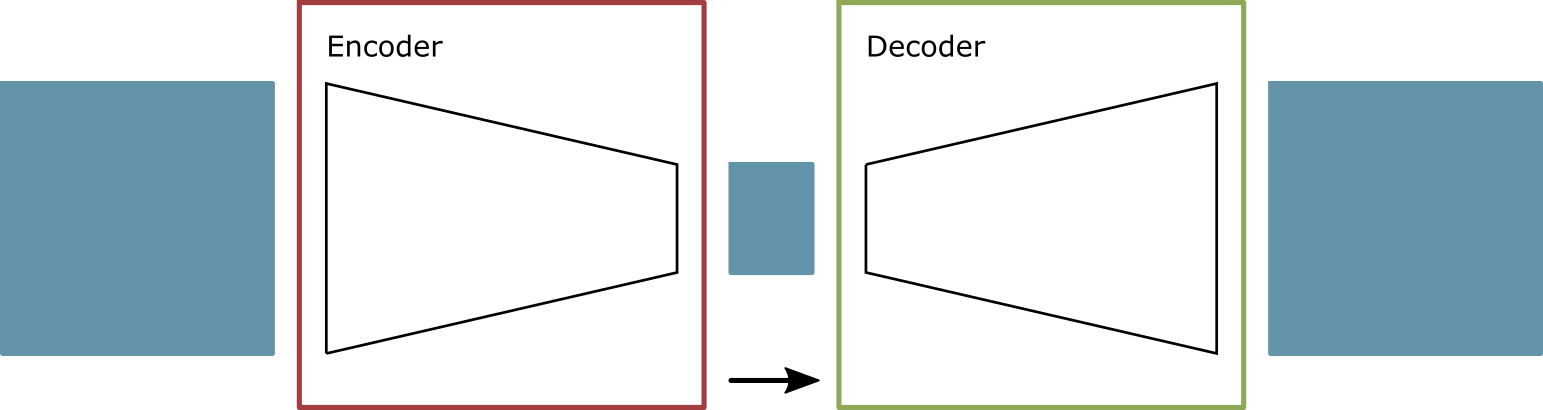
\includegraphics[width=\textwidth]{figure/general-autoencoder.png}
    \caption{Simple autoencoder architecture, which is used in this work. Encoder and decoder are FCNs. Data flow is highlighted to blue. Features in the middle have more channels but less height and width than original image, and this hidden representation takes less space than initial image.}
    \label{autoencoder}
\end{figure}

\subsection{Autoencoder training}

We can train this autoencoder by minimizing L1 \ref{eq:1} and L2 \ref{eq:2} distance losses. This is a general pipeline for training autoencoder for image compression. Usually other terms are added to the final loss. But even using this simple pipelines we can still reach a reasonable results \ref{autoencoder-result}.

\begin{figure}[!ht]
    \centering
    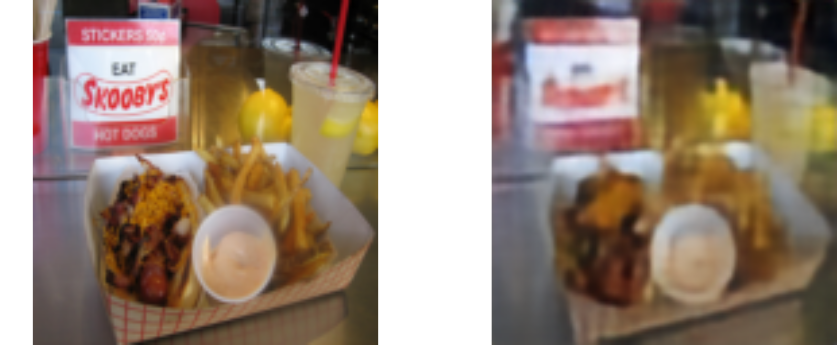
\includegraphics[width=\textwidth]{figure/autoencoder-result.png}
    \caption{Results obtained by training simple autoencoder. (left) Original image, (right) Image obtained after encoding and decoding  using FCN encoder and decoder.}
    \label{autoencoder-result}
\end{figure}

L2 distance loss can be obtained using formula below \ref{eq:2}

\begin{equation}
    \label{eq:2}
    L2=\sum (\hat{I}-I)^2
\end{equation}

Having hidden features (or latents), we can then compress them using one of lossless algorithms such as arithmetic coding or even Huffman coding algorithms. Since we have numerical values here, arithmetic coding is more preferable.

It is possible to use another autoencoder to encode latents obtained from the encoder into hyperlatents, that will have even smaller dimensionality, and apply arithmetic coding to these hyperlatents. We are using a Hyperprior module, which was described in \cite{Ballé_Minnen_Singh_Hwang_Johnston_2018}

\begin{figure}[!ht]
    \centering
    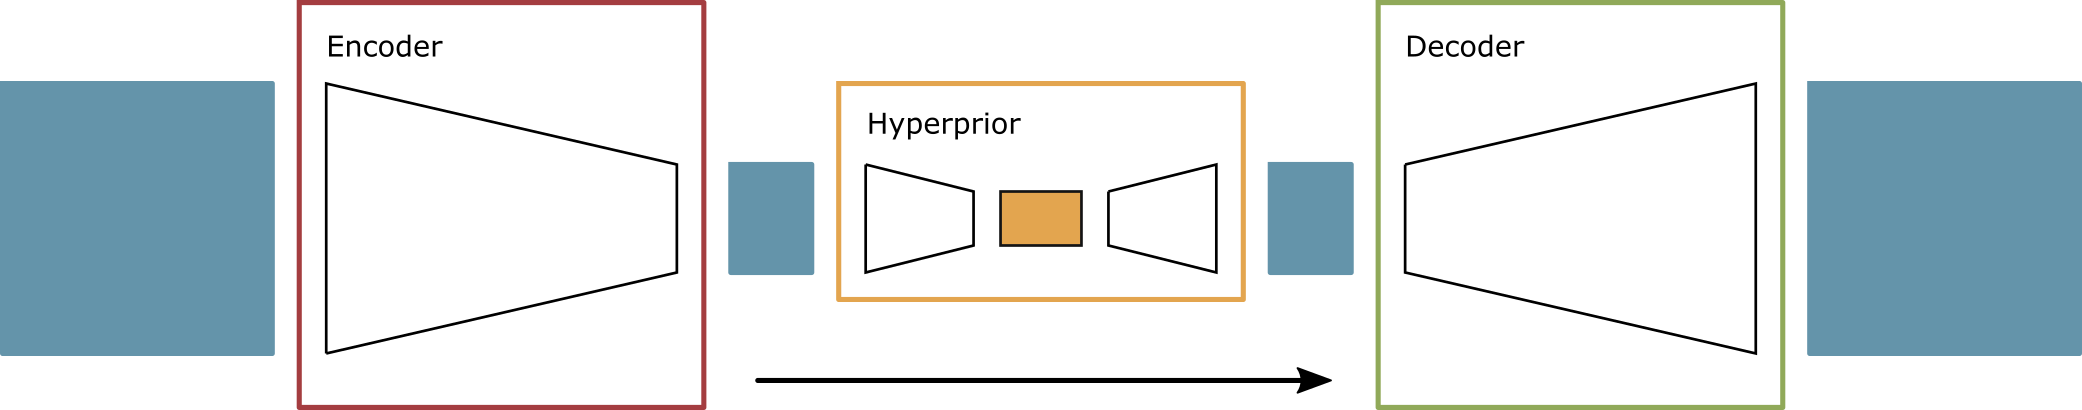
\includegraphics[width=\textwidth]{figure/general.png}
    \caption{Compression general pipeline. Encoder is used to obtain latents, then another encoder is used to obtain hyperlatents. Yellow block is quantization and arithmetic coding block. Then hyperlatents are decoded to latents and the last step is to pass it though Decoder to obtain reconstructed image.}
    \label{whole-system-geneal-pipeline}
\end{figure}

\section{Coding}

The last step of compression is coding. Coding is lossless, and basically it is an independent algorithm. Usually arithmetic coding is used.

Arithmetic coding is a form of entropy coding \ref{arithmetic_coding}. It is lossless, which means that after compression and decompression no information is lost. It is used to compress numeric sequencies, which makes it perfect for the task of image compression since after quantization process we have exactly what is required - a list of integers. According to Shannon's source coding theorem an optimal representation converges to $log_2P$ bits per symbol for a symbol with frequency $P$.

The first step of arithmetic coding is building of probability information from source sequence. After knowing all the probabilities we need to place them according to their probabilities. Then the range of the first symbol is set to be a next range. Then the process is repeated $N$ times, where $N$ is a length of sequence. By the end of this process we have a single segment in the global range (on the \ref{arithmetic_coding} it is the range from $0.534$ to $0.54$). Then we just pick a number from this range. This number is a compressed sequence.

\begin{figure}[!ht]
    \centering
    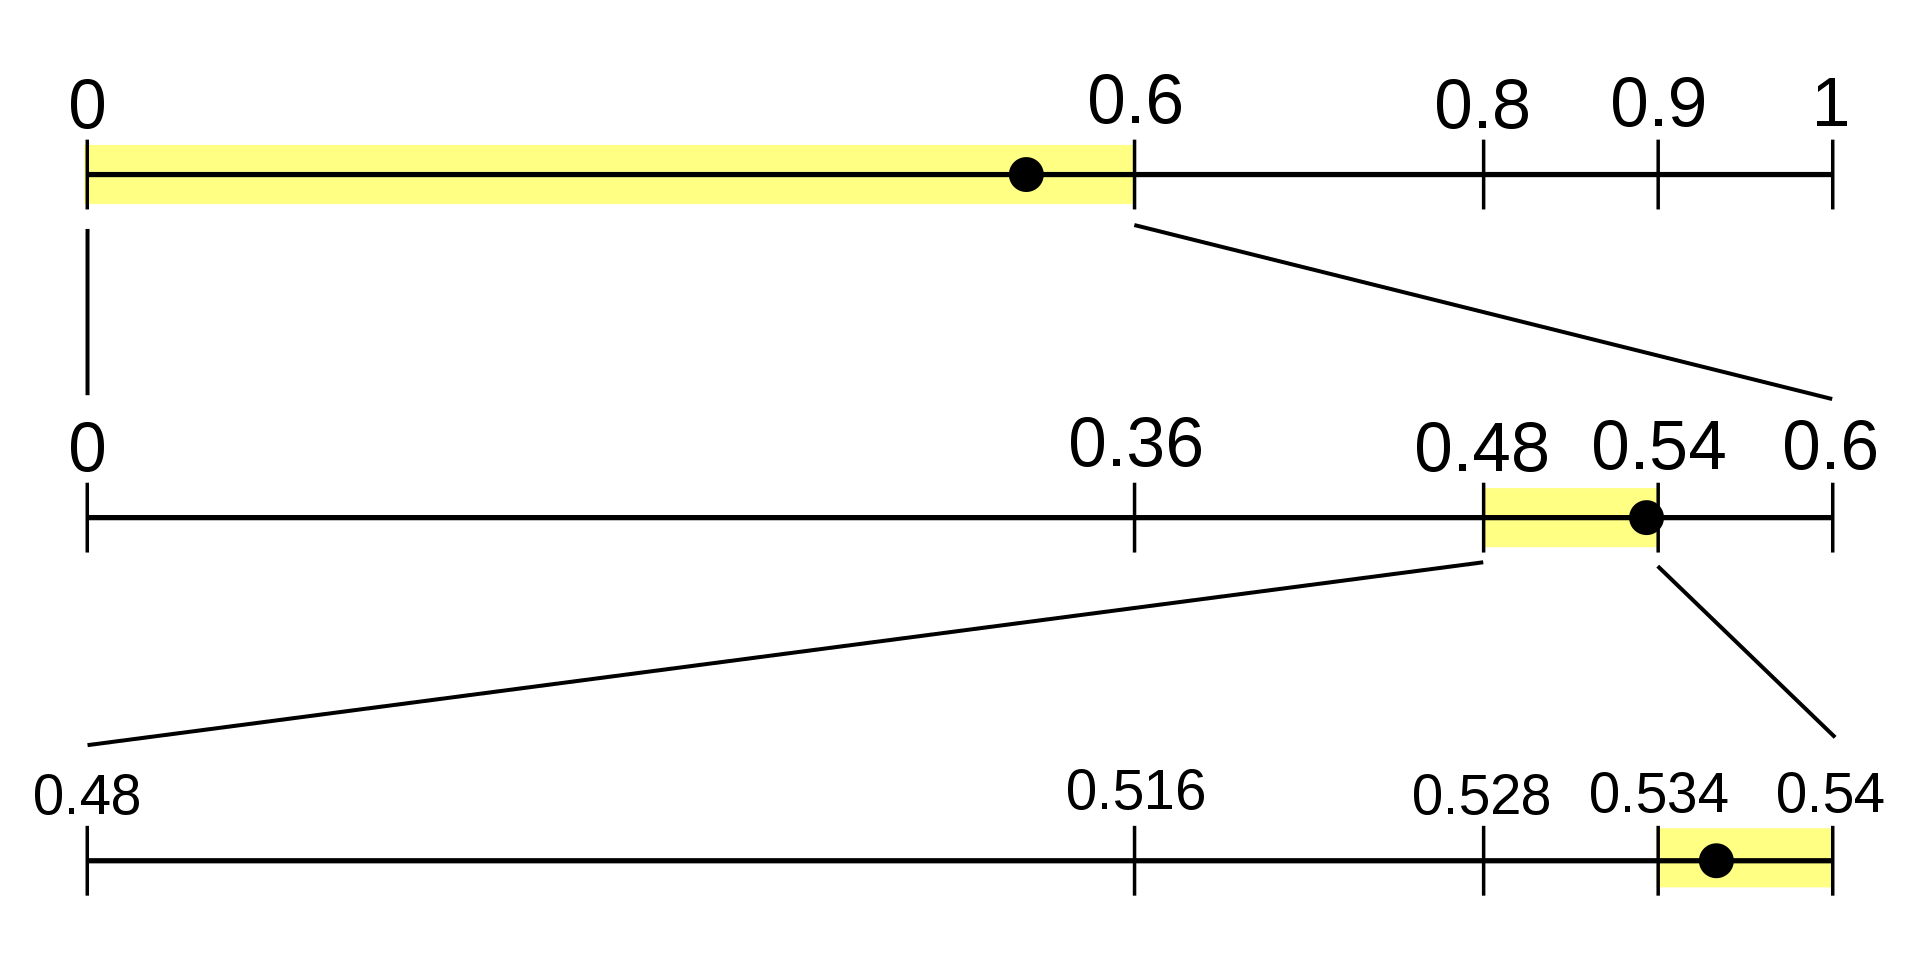
\includegraphics[width=\textwidth]{figure/Arithmetic_encoding.svg.png}
    \caption{Arithmetic coding for a sequence with length 3. Each horizontal segment represents a position in sequence, and parts of these segments correspond to probabilities or frequencies of the symbols they are related to.}
    \label{arithmetic_coding}
\end{figure}

Compressed sequence is stored as a single number. It's also required to remember probabilities since they are used in decompression process.

\section{GAN training pipeline}

Generative adversarial networks (GANs) show a great performance in training generative models. For GANs training pipeline is slightly different from traditional deep learning pipeline. In \cite{Goodfellow_Pouget-Abadie_Mirza_Xu_Warde-Farley_Ozair_Courville_Bengio_2014} they introduced a neural network training pipeline with two networks: generator and discriminator. Generators objective is to produce a good enough synthetic data. Discriminators objective is to find out, whether given sample synthetic or real. So, trained generator network can be used then to solve a problem.

\section{Training}

Training in Machine Learning is a process of adjusting model parameters based on selected criteria and according to one of selected training algorithms. Conceptually training of Machine Learning model is based on the following logic: we can input a data sample to the model, then we have an output, which we should judge by calculating a criteria. We call such a criteria loss. Loss is a function with network output as an input for this function and some number as an output. The process from input to calculating the loss is called a forward pass. We call it forward pass because the calculations, which are happening all the way from input to the output go from input layers forward to output layer (from first to last).

Let us consider a single forward pass. We have an input of certain dimension $H \times W \times C$, we pass it through encoder, which is a convolutional neural network with output of another dimensions $H' \times W' \times C'$, such that $H' < H$, $W' < W$ and $C' > C$. Basically, after passing input through encoder, we get an intermediate representation with spacial dimensions($H'$ and $W'$) less than input spacial dimensions and much greater channel dimension ($C'$). Afterwards we pass these intermediate features with dimensionality $H' \times W' \times C'$ to decoder convolutional network. Usually decoder uses some kind of deconvolution operation. So, basically decoder takes an input with smaller spatial dimensionality and greater channel dimensionality ($H' \times W' \times C'$), producing an output with greater spatial dimensionality and smaller channel dimensionality ($H'' \times W'' \times C''$), such that $H'' > H'$, $W'' > W'$ and $C'' < C'$. Moreover, the decoder output dimensionality is equal to the encoder output dimensionality ($H'' = H$, $W'' = W$ and $C'' = C$).

After forward pass we calculate a loss. Loss can be any function that can precisely enough calculate how good the model performs. Loss can be a linear combination of functions that measure separate objective separately. As an example we can take a just an $L1$ distance between the input $I$ and the output $\hat{I}$ of a model \ref{eq:l1}. Each loss function judges performance its own way. For example, if we compare $L1$ and $L2$ \ref{eq:2}, $L1$ can be negative and $L2$ can not. Loss functions are a big subject of researches by themselves. To define a loss means to define a criteria we'll be optimizing, trying to make it as small as it possible, so this criteria should decay with increasing performance of the output.



\begin{equation}
    \label{eq:l1}
    L1=\sum{I-\hat{I}}
\end{equation}

After calculating a loss of the model output we need to adjust model parameters based on what loss function returns. Loss funciton returns a number which can be treated as a degree of deviation from desired $0$ loss value (or, it may be customized to be another number). Once we know how far we are from desired output we start propagating this output back from the last layer of decoder to the very first layer of the encoder. This process is called a backpropagation. Backpropagation is a way of spreading gradients back through the network, and adjusting each of network parameters based on these gradients.

Backpropagation is a process of sequential gradient propagation. To propagate through a network we need to propagate gradient through each layer starting from the last one and ending through the first layer. To propagate gradient back we can use simple rules of algebra.

Gradient of a scalar-valued differentiable function $\nabla f$ of several variables is the vector field (or vector-valued function) $f$ of whose value at a point $p$ is the vector whose components are the partial derivatives of $f$ at $p$. That is, for $f\colon \mathbb {R} ^{n}\to \mathbb {R}$ its gradient $\nabla f\colon \mathbb {R} ^{n}\to \mathbb {R} ^{n}$ is defined at the point $p=(x_{1},\ldots ,x_{n})$ in n-dimensional space as the vector \ref{eq:gradient}

\begin{equation}
    \label{eq:gradient}
    \nabla f(p)={\begin{bmatrix}{\frac {\partial f}{\partial x_{1}}}(p)\\\vdots \\{\frac {\partial f}{\partial x_{n}}}(p)\end{bmatrix}}
\end{equation}

The nabla symbol $\nabla$ denotes the vector differential operator.

The gradient vector can be interpreted as the "direction and rate of fastest increase". If the gradient of a function is non-zero at a point p, the direction of the gradient is the direction in which the function increases most quickly from p, and the magnitude of the gradient is the rate of increase in that direction, the greatest absolute directional derivative. Further, the gradient is the zero vector at a point if and only if it is a stationary point (where the derivative vanishes). The gradient thus plays a fundamental role in optimization theory, where it is used to maximize a function by gradient ascent.


TODO: furmulas of backpropagation

To train such a system we need two losses: discriminator loss and generator loss. Discriminator loss will penalize discriminator network for it's wrong classification results. The loss we are using in this work is non-saturating loss \ref{eq:loss-g} and \ref{eq:loss-d}, which is just a stable variation of standard GAN loss function. It maximizes the log of the discriminator probabilities.

\begin{equation}
    \label{eq:loss-g}
    \mathcal{L}_G=E_{y\sim p_Y}[-log(D(G(y,s),s))],
\end{equation}

\begin{equation}
    \label{eq:loss-d}
    \mathcal{L}_D=E_{y\sim p_Y}[-log(1-D(G(y,s),s))]+E_{x\sim p_X|s}[-log(D(x,s))]
\end{equation}

The formula above has a following intuition: instead of minimizing a probability of images being fake, it maximizes a probability of images being real, which leads to more stable weight update mechanism.

Since our work is about image compression, we also need to introduce an image compression term in our loss function \ref{eq:loss-eg}. This term is a combination of two values: compression rate loss, which states for a good compression rate of given image and distortion rate, which states for a good quality of reconstructed images. The second term helps to reduce a noise in generated images.

\begin{equation}
    \label{eq:loss-eg}
    \mathcal{L}_{EG}=E_{x\sim p_X}[\lambda r(y)+d(x, x')]
\end{equation}

We can merge \ref{eq:loss-g} an \ref{eq:loss-eg} into one single formula \ref{eq:loss-egp}.

\begin{equation}
    \label{eq:loss-egp}
    \mathcal{L}_{EGP}=E_{x\sim p_X}[\lambda r(y)+d(x, x')-\beta log(D(x',y))]
\end{equation}

So at the end our compression model has two terms, which is exactly the number of terms we want to have while training GAN, since GAN training is performed by incrementally repeating training steps of generator and discriminator. So, we use \ref{eq:loss-egp} during generator train step and we use \ref{eq:loss-d} during discriminator train step.

So, this pipeline describes whole number of actions we need to perform in order to train image compression model. However, images obtained from such model have some unnecessary drawbacks, one of which is the fact that they are blurry \ref{forest-blurry}.

\begin{figure}[!ht]
    \centering
    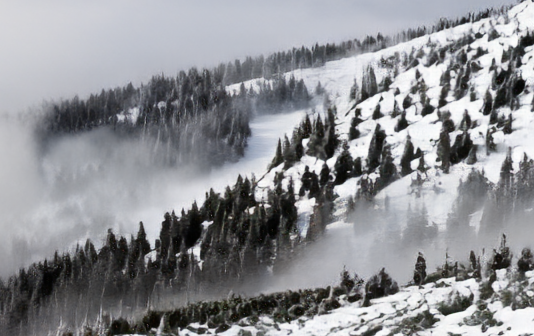
\includegraphics[width=\textwidth]{figure/forest-blurry.png}
    \caption{Example of an image compressed with Hyperprior module.}
    \label{forest-blurry}
\end{figure}

To overcome this issue we propose a novel approach: we include several super resolution layers in our generator. These layers remove blurry artifacts and make resulting images more sharp.

Image super resolution proposal can be formulated as a learning complex degradations from data. It is clear that the first step here is to produce a dataset from that a model then can be learned. Common choice here is to apply degradations on images before passing them into training pipeline.

We consider following degradations: blur, noise, downsampling, JPEG compression. Blur makes image less sharp and here traditional choice is gaussian blur kernel. Noise increases variance of image pixels, common choice is gaussian noise, which is sampled from gaussian distribution. Downsampling operation makes an mage smaller. There are several approaches to resize images: bilinear, bicubic and nearest neighbor interpolation.

For super resolution we use a common architecture, which has been used in \cite{Ledig_Theis_Huszar_Caballero_Cunningham_Acosta_Aitken_Tejani_Totz_Wang_et_al_2017}, \cite{Wang_Yu_Wu_Gu_Liu_Dong_Qiao_Loy_2019}, \cite{Wang_Xie_Dong_Shan_2021}. This architecture also is a fully convolutional net. Here we use a deep convolutional network body to extract meaningful features from an image (this network is 23 layers deep currently). We use residual connections for each layer of the network body. Each residual block performs four convolution operations, having features concatenated with all previous outputs channel-wise \ref{upscale}.

\begin{figure}[!ht]
    \centering
    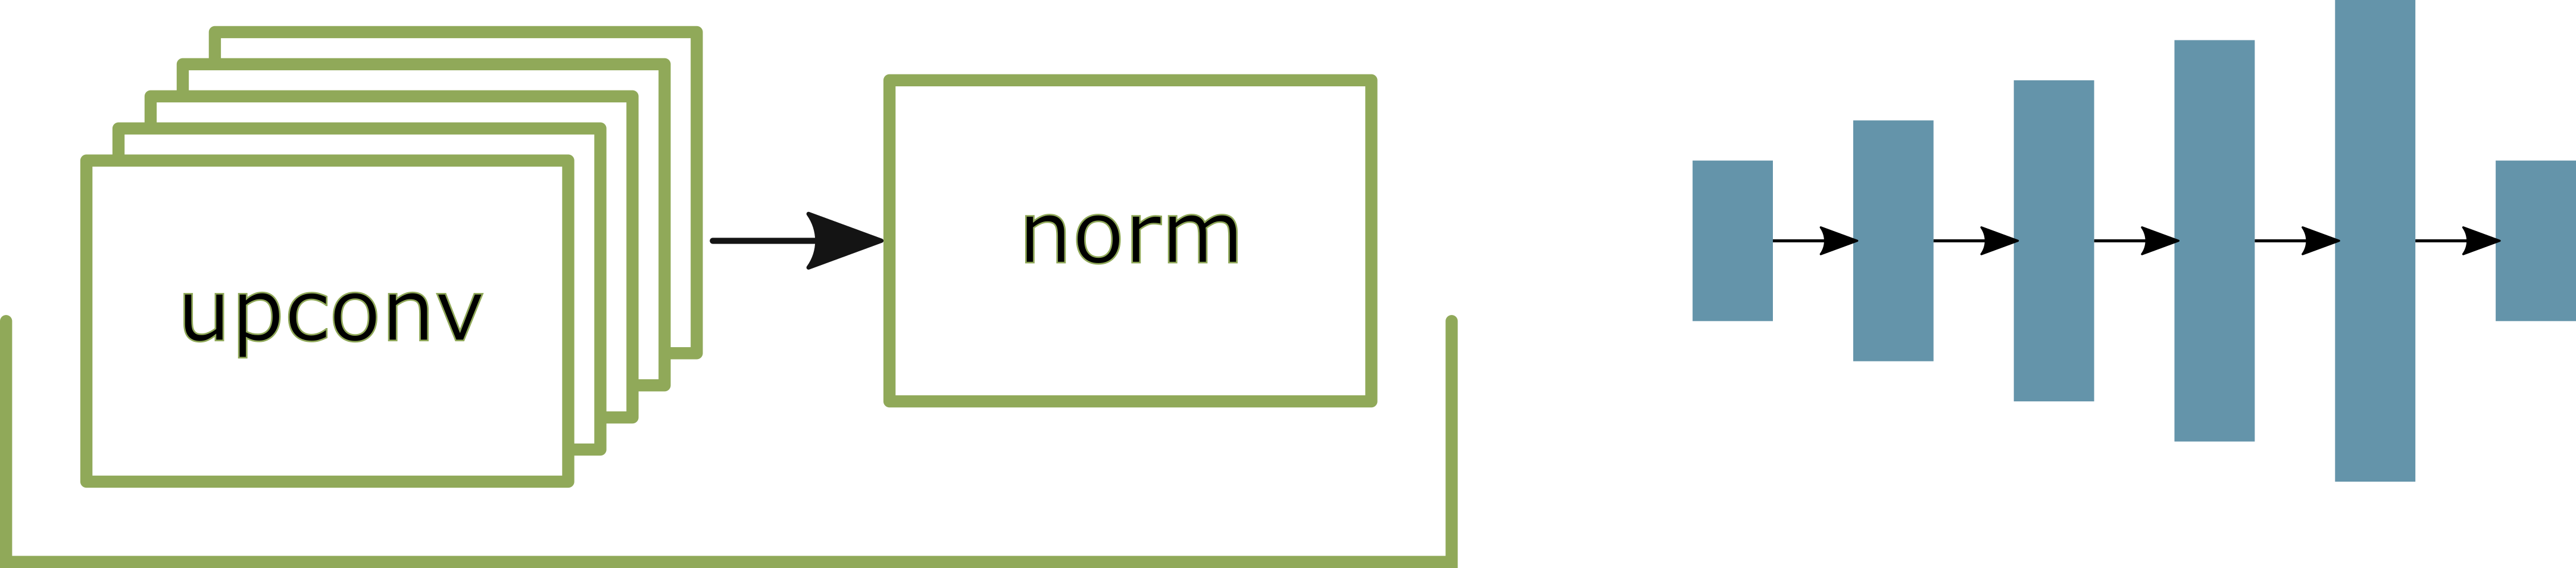
\includegraphics[width=\textwidth]{figure/upscale.png}
    \caption{For upscale we use a combination of convolution layers with residual connection (left). For visualization we also include channel dimensionality dynamics along the propagation through the convolutional layers (right).}
    \label{upscale}
\end{figure}

Having convolutional features propagated through the network body we apply two simple upsampling layers, that use a non-learnable interpolation operation and convolution layer followed by ReLU activation function.

We imply L1 loss \ref{eq:1}, L2 loss \ref{eq:2} and GAN loss \ref{eq:loss-d}, \ref{eq:loss-g} to pretrain super resolution module. Afterwards we fine tune an entire framework. Using same loss functions mentioned above.

\chapter{Experiments}

We train our networks on datasets described in \nameref{section:data}. We set $\lambda$ to $1$ and $\beta$ to $0.15$ parameters from \ref{eq:loss-g}. We set a learning rate of $10^{-4}$ and train the network using Adam optimizer. We train the networks in 2 steps: first step is training compression and upscale networks in GAN manner (using generator and discriminator losses), the second step is to fine tune them together.

\begin{figure}[!ht]
    \centering
    \includegraphics[width=\textwidth]{figure/pictures.png}
    \caption{Results of image decompression. Original image is (left), image compressed without upscale module is (middle) and image compressed with upscale module is (right).}
    \label{road}
\end{figure}

By increasing and decreasing $\beta$ and $\lambda$ we can control a tradeoff between compression and distortion loss trams on the training stage. This allows us to select a better hyperparameter for the network. The process of hyperparameter selection is following: start training network and after some number of iterations (we usually wait few epochs) we compare the results of validation dataset. If this set of hyperparameters performs better than previous set, we should use this one. It is clear from \ref{compession-losses}, how compression and distortion losses in combination together give final loss term \ref{eq:loss-egp}.

\begin{figure}[!ht]
    \centering
    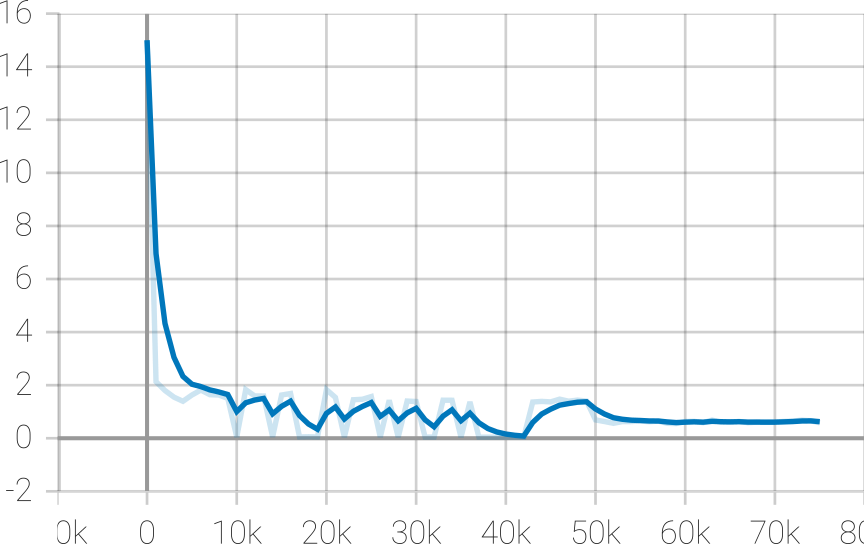
\includegraphics[width=0.3\textwidth]{figure/weighted_compression_weighted_rate.png}
    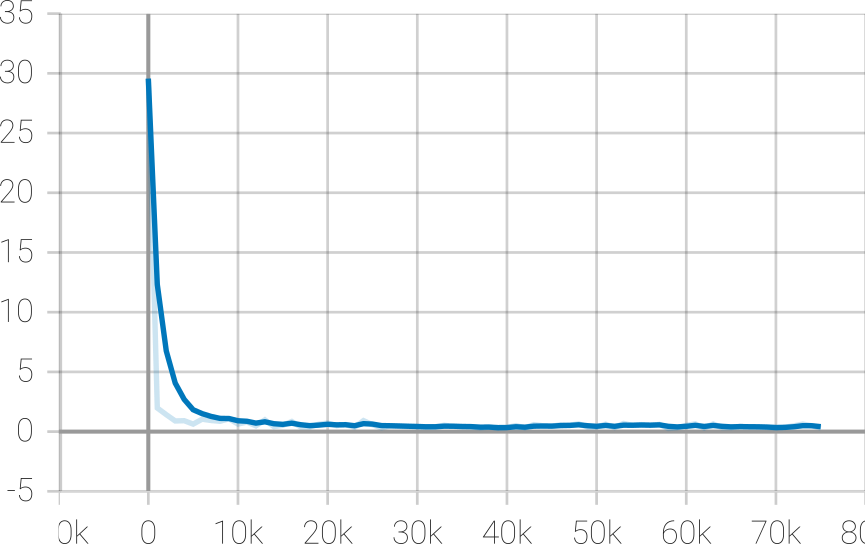
\includegraphics[width=0.3\textwidth]{figure/weighted_compression_weighted_distortion.png}
    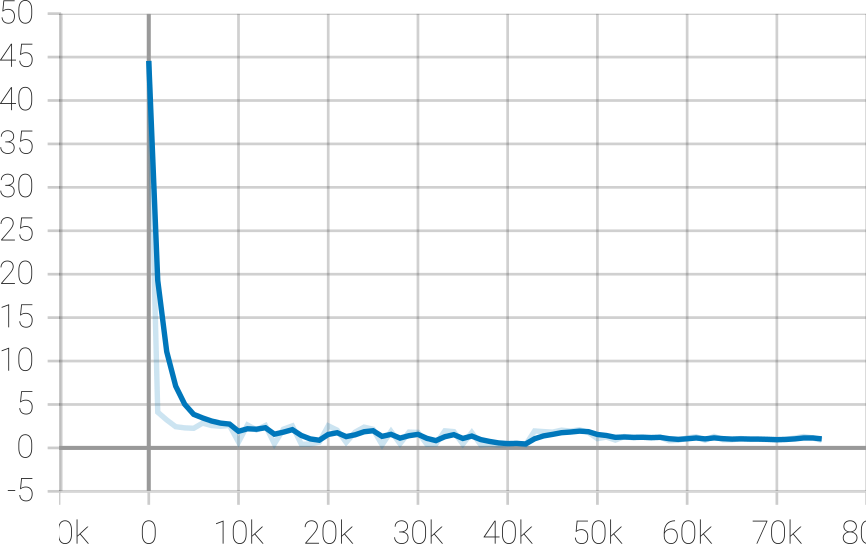
\includegraphics[width=0.3\textwidth]{figure/weighted_compression_weighted_R_D.png}
    \caption{Training process for compression module. As we can see, compression rate term (left) and distortion term (middle) in combination give final rate/distortion loss (right).}
    \label{compession-losses}
\end{figure}

We still do not have enough metric to plot many charts. We figure out, however, that compressed image takes less than 3 times space than JPEG compressed image.

\chapter{Data}
\label{section:data}

We used several datasets to train and test the models we've implemented. One is Visual Genome dataset, which has been used in many other works \cite{Krishna_Zhu_Groth_Johnson_Hata_Kravitz_Chen_Kalantidis_Li_Shamma_etal_2016}. Visual genome consists of more than 100,000 images labeled with scene graphs. We used Visual Genome for training scene graph based compression models.

Dataset consists of several main parts:

\begin{enumerate}
    \item Region descriptions. Human labeled important regions of an image, each description phrase is 1 to 16 words long.
    \item Objects. Objects labeled and canonicalized to a synset ID in WordNet.
    \item Attributes. Both images and objects have attributes. They are also canonicalized to WordNet.
    \item Relationships. Connects a pair of objects. Relationships are directed.
    \item Region graphs. A graph of a region of an image. These could be more than one region graph on one image.
    \item Scene graphs. A composition of region graph of an image. One image has exactly one scene graph.
    \item Question-answer pairs. There are both region-based and freeform QA pairs.
\end{enumerate}

It might be more adequate to split the Visual Genome dataset on the following general parts for better understanding:

\begin{enumerate}
    \item Images in JPEG format with various height and width.
    \item Detected objects information (coordinates of rectangles for each object, objects labels, objects attributes).
    \item Scene graphs, obtained from images.
\end{enumerate}

The dataset itself is quite big (more then 30 Gb), so we implemented a data loader that can work with such amounts of data. There were some efforts \cite{Yang_2018_Graph} to build a framework capable of working with the Visual Genome dataset, however there are no any stable version to work with.

Another dataset we are using in this work is Open Images dataset \cite{OpenImages2}, which is a a huge dataset of 9 million images. Those images are annotated with image-level and object-level annotations, bounding boxes, visual relations and segmentation masks. We use this dataset to train and test models of image compression, which means we do only need clean images without annotations. We use near 150,000 images subset from 9,000,000 images dataset. This amount is sufficient to train a compression model.

\chapter{Future work}

Future work mainly incudes improvements of Generator network. We plan to reduce number of layers in generator by applying the same backbone network to both upscale and deconvolution networks. This will help to reduce a number of training and fine tuning iterations and help to reduce number of parameters, which will directly affect portability of the network to devices with small GPU. We also think that by improving a backbone we can increase an accuracy of reconstructions and resolve a false textures issue, but it still needs to be tested.

There also is an issue with metics for this work. For the final thesis we need to collect metics that will reflect three aspects of our complex network:

\begin{enumerate}
    \item Compression ratio. We plan to use traditional BPP (bits pe pixel) metic, since this number can show the effectiveness of compression.
    \item Reconstructed image distortion. We plan to use a distance between images for this metric. In combination with PSNR (pike signal to noise ratio) it can reflect similarity between original and reconstructed image.
    \item Upscale image quality. Since we also include upscale layers, it's important to measure a quality of upscale images. Unfortunately, it is not possible to directly measure, how good upscale operation performs, however we consider traditional tick, such as downsizing initial image before training.
\end{enumerate}

\chapter{Schedule and arrangement}

Proposed architecture has a compound structure. As it has been mentioned above, the architecture can be separated into two major parts: encoder and decoder part. From our experiments we see that encoder part performs good and there is no need to improve it. However, decoder part is a bit too heavy and complicated. We plan to improve it and reduce number of parameters.

We refer to the schedule from thesis proposal \ref{tab:schedule}.

\begin{table}
    \centering
    \caption{Schedule}
    \label{tab:schedule}
    \begin{tabular}{p{4cm}|p{8cm}|p{2cm}|p{2cm}}
        \hline
        Task                    & Description                                                                                                                                & Deadline    & Status      \\
        \hline
        Build a model prototype & Build a first version of a model that is capable to compress and restore images, it will include building and training encoder and decoder & September 1 & Done        \\
        \hline
        Improve model prototype & Adjust parameters, decide on additional convolutional features size                                                                        & December 1  & Done        \\
        \hline
        Research proposal 1     & Reduce number of layers in generator                                                                                                       & February 1  & In progress \\
        \hline
        Research proposal 2     & Solve false textures issue                                                                                                                 & March 1     & In progress \\
        \hline
        Write the final thesis  & Summarize research in the final thesis                                                                                                     & May 20      & In progress \\
        \hline
    \end{tabular}
\end{table}

Tasks in this table are not really concrete. So it's more like a template for future planning. We are using Trello software to deal with concrete short-term tasks. Time management however is not a part of a technical part of the project, so we just mention it here.